
\chapter{Pattern Recognition for Seizure Prediction}
\label{ch:2deterministic}
The field of pattern recognition includes designing pipelines to learn from data, represented as feature vectors, and recognize patterns which generalize across past and future data. A considerable amount of research has revealed that, indeed, machine learning classifiers are able to perform above-chance classification between preictal and interictal feature vectors in many patients.

Previously, the success of these methods for seizure prediction based on intracranial EEG has been demonstrated \cite{mirowski2009classification, kaggle2014contests} in human patients as well as animals. In this chapter, we show that similar results can be achieved by the same methods applied to scalp-surface EEG.


\section{Methods}
We follow closely the exploratory methods demonstrated in \citet{mirowski2009classification}. They show applications of several classifiers to seizure prediction. Bivariate feature extraction methods are used to create 2-d patterns for classification of preictal and interictal patterns (cf. figure \ref{fig:c2:nlid}).


\subsubsection{Data collection and specification}

Typical publicly available epilepsy-seizure-prediction datasets consists of long-term raw EEG recordings from pre-sugical evaluation periods, supplemented with annotations provided by approved experts \cite{handa2021open}. In these datasets, the occurrence of seizures is reported as a list of ictal (seizure) intervals
\begin{equation}
    I := \{Ictal_i\} = \{\bra{t_{start}^i|S_i|t_{end}^i} \ket{}\}
\label{eq:define_ictal}
\end{equation}
where $t_{start}$ is the seizure onset, $t_{end}$ the seizure offset, and $S_i$, when available, are the additional details reported such as epilepsy etiology, seizure type classification.
In this project, we used data from the Epilepsiae Dataset \cite{ihle2012epilepsiae}. Table \ref{table:data} lists raw recording length, sample frequency, number of surface electrodes and size-on-disk per patient.


\begin{table}[h]
\centering
% increase table row spacing, adjust to taste
\renewcommand{\arraystretch}{1.3}

% if using array.sty, it might be a good idea to tweak the value of
% \extrarowheight
\caption{Data used in this chapter.}
\label{table:data}

% % Some packages, such as MDW tools, offer better commands for making tables
% % than the plain LaTeX2e tabular which is used here.
\begin{tabular}{|c|c|c|c|c|}
\hline
\textbf{Patient Name} & \textbf{Length} & \textbf{Frequency} & \textbf{Electrodes} & \textbf{SOD} \\
\hline
\verb|pat_3500| & 92.8 h & 1024 Hz & 32 & \texttt{21 GB} \\
\hline
\verb|pat_3700| & 79.8 h & 512 Hz & 32 & \texttt{8.8 GB}\\
\hline
\verb|pat_7200| & 94.6 h & 1024 Hz & 29 & \texttt{21 GB}\\
\hline
\end{tabular}
\end{table}


\subsection{Preprocessing}
Although it is common to apply spectral filters to EEG data to reduce line noise etc., we chose to focus on the effect of classifier and features choice on predictive performance, and thus kept preprocessing to a minimum.
First, EEG channel selection was performed to select a spatially far-reaching distributed subset of 19 channels, common to all patients (see figure \ref{fig:c2det:channellocs}).



\begin{figure}[h]
    \centering
    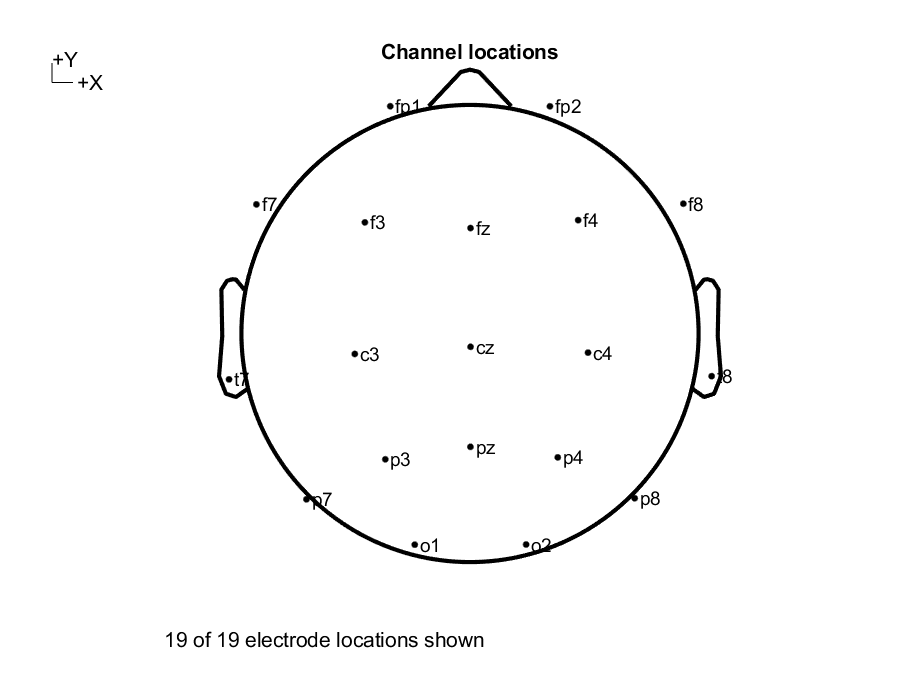
\includegraphics{c2Deterministic/Figs/PSP/topomap.eps}
    \Caption{EEG channel locations used in this chapter}{\begin{texttt}
    The common set of channels ['Fp1', 'Fp2', 'F3', 'F4', 'C3', 'C4', 'P3', 'P4', 'O1', 'O2', 'F7', 'F8', 'Fz', 'Cz', 'Pz', 'T7', 'T8', 'P7', 'P8'] was selected for all patients.
\end{texttt}.}
    \label{fig:c2det:channellocs}
\end{figure}

This was done to reduce data dimension as well as standardization amongst patients.
The raw data was resampled to 256 Hz to reduce disk space and processing time.


\subsection{Preictal and Interictal Binarization}
\label{c2:labeling}
A practical way to characterize time-varying signal dynamics is through a sliding window approach (see Fig. 1. in \cite{lehnertz2017capturing}). An EEG time series matrix $X$ is partitioned temporally into non-overlapping windows $x_1, ..., x_N$. Each window $x_i$ is given a label $y_i$, to form a dataset $D = \{(x_1, y_1),...,(x_N,y_N)\}$. Optionally, each window is transformed via a feature extraction function $f(x)$, which yields a feature-formed dataset $D_f = \{(f(x_1), y_1),...,(f(x_N),y_N)\}$.

\begin{definition}[Preictal state]
The state of preceding a seizure by a short time (minutes to hours).
\end{definition}

\begin{definition}[Interictal state]
The state of being at least a few hours before and after a seizure.
\end{definition}

Hence, each EEG window $x_i$ is checked for distance to the provided seizure labels (see eq. \ref{eq:define_ictal}) to create the appropriate label:
\begin{equation}
    y_i := 
      \begin{cases}
    0 & \text{if $preictal(x_i)$} \\
    1 & \text{if $interictal(x_i)$} \\
  \end{cases}
\end{equation}

Formally, $ictal(x_i)$ if and only if $x_i$ temporally overlaps some ictal interval $I_j$. Similarly, $preictal(x_i)$ if and only if $x_i$ overlaps with some $\tau_P$ time interval preceding an ictal interval $I_j$. Finally, $interictal(x_i)$ if and only if $x_i$ does not closely precede or proceed any seizure interval, with thresholds $\tau_{a}$ before and $\tau_{b}$ after, respectively. In this chapter, $\tau_{a}$ and $\tau_{b}$ are each taken to be 4 hours, and $\tau_P$ is taken to be 1 hour, in line with previous works and competitions such as \citet{mirowski2009classification, kaggle2014contests}.


\subsection{Bivariate Feature Extraction Methods}
\label{sec:c2:features}
The deterministic classification method relies on hand-crafted, manually engineered, features. Specifically, following \cite{mirowski2009classification}, we focus on bivariate measures of synchronicity between pairs of EEG channels (see figure \ref{fig:c2:pca_features} for examples).


\begin{figure}[htb]
    \centering
    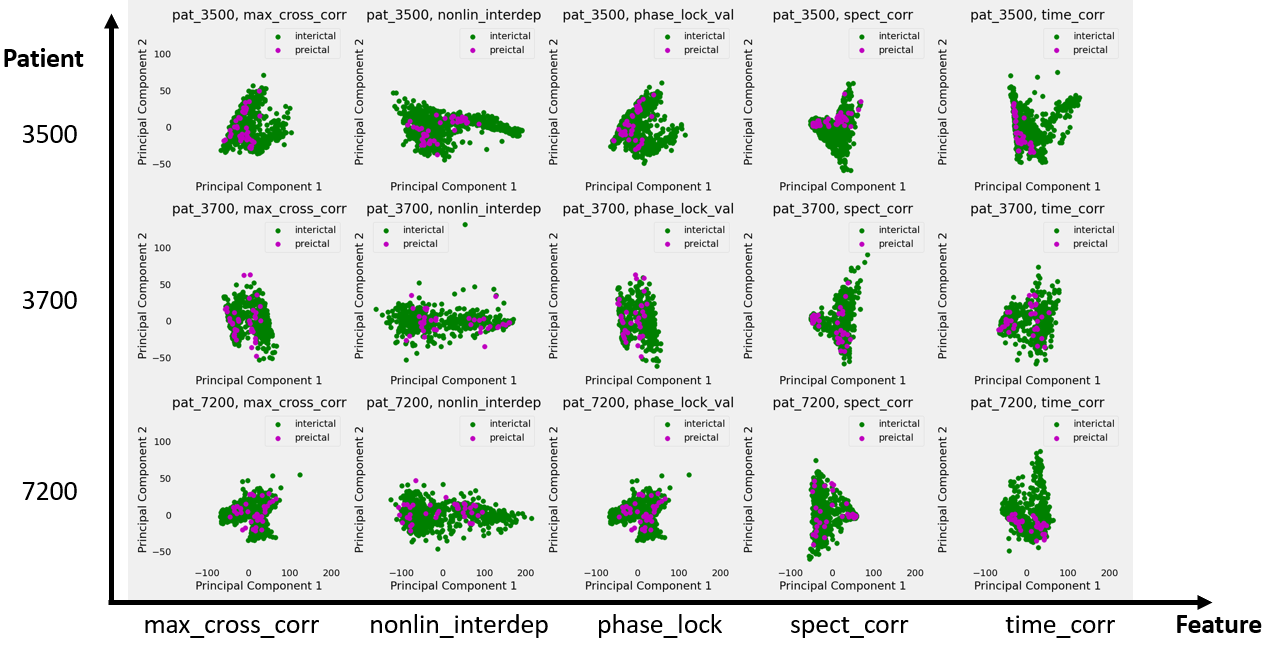
\includegraphics[width=\textwidth]{c2Deterministic/Figs/PSP/pca_features_patients2.png}
    \Caption{First 2 principal components of transformed data per patient and feature type}{The feature types are (left to right): maximal linear cross correlation, nonlinear interdependence, phase locking value, spectral domain correlation, time domain correlation. Each point represents a flattened 5-minute window (i.e., a pattern), and it's color denotes class label (interictal or preictal).}
    \label{fig:c2:pca_features}
\end{figure}

For each patient, the recording is segmented into 5 minute windows. At loading time the EEG was shifted and scaled to zero mean and unit standard deviation, per 5-minute window. Each window is segmented into 60 frames, each 5 seconds long. Each 5 second frame is reduced into a vector of length $c \cdot (c - 1) / 2$ (where $c$ is number of channels), via one of the feature extraction methods described below. Each 5 minute window is regarded a single pattern with a single label (preictal vs. interictal).


\subsubsection{Maximal Linear Cross Correlation (figure \ref{fig:c2:max_line_corr})}
In order to quantify the similarity of two signals $\{x_i\}$ and $\{y_i\}$ the maximum of a normalized cross-correlation function is taken as a measure for lag synchronization \cite{rosenblum1997phase}:

\begin{equation}
    C_{max} = \max_{\tau \in [-N,N]}{ \abs{ \frac{C_{xy}(\tau)}{\sqrt{C_{xx}(0) \cdot C_{yy}(0)} }}}
\end{equation}

Where
\begin{equation}
    C_{xy} = \begin{cases}
        \frac{1}{N-\tau}\sum_{i=1}^{N-\tau}x_{i+\tau}y_i, & \text{for } \tau >= 0\\
        C_{yx}(-\tau), & \text{for } \tau < 0
        \end{cases}
\end{equation}

is the linear cross-correlation function. $C_{max}$ is confined to the interval $[0,1]$ with high values indicating that the two signals have a similar course in time (though possibly shifted by a time lag $\tau$) while dissimilar signals will result in values close to zero.

\begin{figure}[htb]
    \centering
    \begin{subfigure}[t]{0.4\textwidth}
        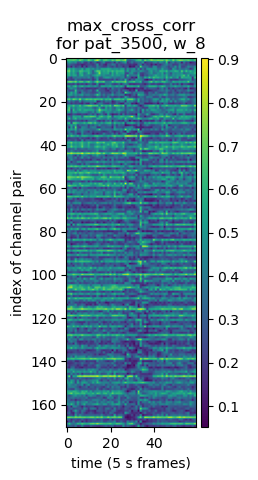
\includegraphics[width=\textwidth]{c2Deterministic/Figs/PSP/max_cross_corr.png}
        \caption{Maximal Linear Cross-Correlation}{}
        \label{fig:c2:max_line_corr}
    \end{subfigure}
    \begin{subfigure}[t]{0.4\textwidth}
    \hfill
        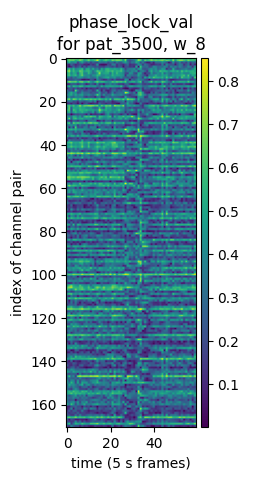
\includegraphics[width=\textwidth]{c2Deterministic/Figs/PSP/phase_lock_val.png}
        \caption{Phase Locking Value}{}
        \label{fig:c2:plv}
    \end{subfigure}
    \Caption{Two types of bivariate features}{Here are shown example patterns created by transforming 19-channel EEG recordings of length 5 minutes into maximal linear cross correlation (a) and phase locking values (b). Each row represents the feature values for a pair of channels, and each column represents those values for a particular 5 second frame. The frames are concatenated to form the window.}
    \label{fig:c2:corr}
\end{figure}



\subsubsection{Phase Locking Value (figure \ref{fig:c2:plv})}
Introduced in \cite{lachaux1999measuring}, the \emph{Phase Locking Value} measures synchronicity between eeg channels in different locations on the scalp. First, for each channel $i$, the instantaneous phase $\sigma_i ^a (t)$ of the analytical signal $x_i^a(t)$ is extracted. Then, for each pair $(i, j)$ of channels, we compute the modulus of the time averaged phase difference mapped onto the unit circle:
\begin{equation}
    PLV_{ij} = \abs{\frac{1}{T}\sum_t e^{i(\phi_i^a(t) - \phi_j^a(t))} }
\end{equation}


\subsubsection{Correlation Coefficients and Eigenvalues in the Time and Frequency Domains (figure \ref{fig:c2:corr})}
We compute the correlation coefficients between each pair of EEG channels, along with the eigenvalues of the correlation coefficients matrix, in both the time and frequency domains.
This provides two more sets of measures of synchronicity across EEG channels.

\begin{figure}[htb]
    \centering
    \begin{subfigure}[t]{0.3\textwidth}
        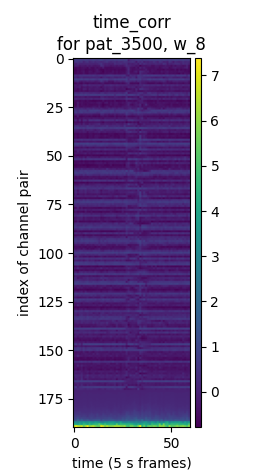
\includegraphics[width=\textwidth]{c2Deterministic/Figs/PSP/time_corr.png}
        \caption{Time-domain}{}
    \end{subfigure}
    \hfill
    \begin{subfigure}[t]{0.3\textwidth}
        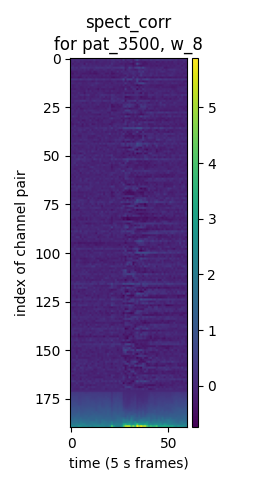
\includegraphics[width=\textwidth]{c2Deterministic/Figs/PSP/spect_corr.png}
        \caption{Spectral-domain}{}
    \end{subfigure}
    \hfill
    \begin{subfigure}[t]{0.3\textwidth}
        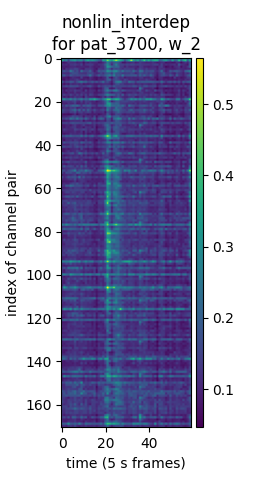
\includegraphics[width=\textwidth]{c2Deterministic/Figs/PSP/nonlin_interdep.png}
        \caption{Nonlinear Interdependence}{}
        \label{fig:c2:nlid}
    \end{subfigure}
    \Caption{Three types of bivariate features}{Example patterns created by transforming 19-channel EEG recordings of length 5 minutes into inter-channel correlation coefficients with eigenvalues appended at the bottom (a and b), and nonlinear interdependence (c).}
    \label{fig:c2:corr_and_nonlin}
\end{figure}

\subsubsection{Nonlinear Interdependence (figure \ref{fig:c2:nlid})}
The \emph{non-linear interdependence} measure for generalized  synchronization between two EEG single-channel signals $\{x_i\}$ and $\{y_i\}$ is presented in \cite{mormann2007seizure}.
First, the two signals are represented as trajectories in a state space, via time-delay embedding. Then, an asymmetric statistic measuring the Euclidean distance, in the reconstructed state-space, between trajectories  $\{\vec{x}_i\}$ and $\{\vec{y}_i\}$ is calculated for each time point. This is done for each pair of channels. See \cite{mirowski2008comparing} for more details.

\subsection{Classifiers}
We trained and tested 9 of classifiers implemented in the \emph{scikit-learn} \cite{sklearn_api} ML toolkit (v1.0.1), listed in table \ref{table:classifiers}. We chose a variety of classifiers from different families (i.e., neural networks, ensembles and decision trees).

\begin{table}[h]
\centering
% increase table row spacing, adjust to taste
\renewcommand{\arraystretch}{1.3}

% \begin{longtable}{ |c|c|c|c| }
% if using array.sty, it might be a good idea to tweak the value of
% \extrarowheight
\Caption{Classifiers used in chapter and their hyperparameter settings}{The settings chosen were the default settings provided by sci-kit learn v.1.0.1. They are repeated here for reference.}
\label{table:classifiers}

% % Some packages, such as MDW tools, offer better commands for making tables
% % than the plain LaTeX2e tabular which is used here.
\begin{tabular}{|c|c|}
\hline
\textbf{Classifier Name} & \textbf{Hyperparameters}\\
\hline
Nearest Neighbors & \texttt{K=3} \\
\hline
Linear SVM & \texttt{kernel="linear", C=0.025}\\
\hline
RBF SVM & \texttt{gamma=2, C=1}\\
\hline
Decision Tree & \verb|max_depth=5|\\
\hline
Random Forest & \verb|max_depth=5, n_estimators=10|\\
\hline
Neural Net & \verb|alpha=1, max_iter=1000|\\
\hline
AdaBoost & \verb|n_estimators=50, learning_rate=1.0, algorithm='SAMME.R'|\\
\hline
Naive Bayes & None\\
\hline
QDA & \verb|reg_param=0.0|\\
\hline
\end{tabular}
\end{table}



\section{Results}
A total of 117 classifier-datasets pairs were trained and evaluated with 5-fold cross validation, yielding a total of 585 model fits. In each fold, the classifier was trained on a random subset of 80\% of the data, and tested on the remaining 20\%.


\subsection{Evaluation Metrics}
We report the following metrics for all features-classifiers pairs:
\begin{enumerate}
    \item ROC AUC
    \item Precision
    \item Recall
    \item fit time
    \item score time
\end{enumerate} 


\subsection{Classifier and Feature Comparison}
Figures \ref{fig:c2:mean_roc_auc} and \ref{fig:c2:std_roc_auc} show the mean and standard-deviation for each classifier on each feature set, for each patient. It is found that the Linear SVM and Neural Net (MLPClassifier) are the top two performers consistently, sometimes followed closely by the Nearest Neighbor Classifier.


\begin{figure}[!htb]
    \centering
    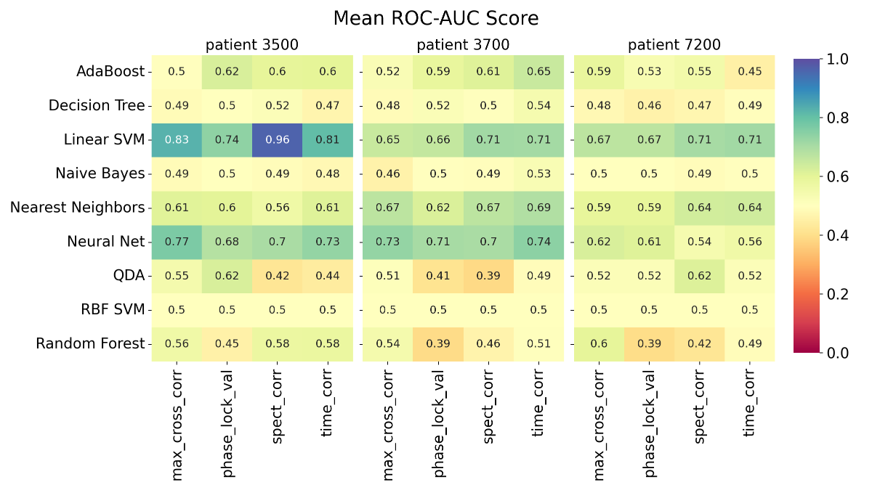
\includegraphics[width=\textwidth]{c2Deterministic/Figs/PSP/mean_roc_auc_classifiers_and_features.png}
    \Caption{Mean AUC-ROC scores for 5-fold cross validation.}{}
    \label{fig:c2:mean_roc_auc}

    \centering
    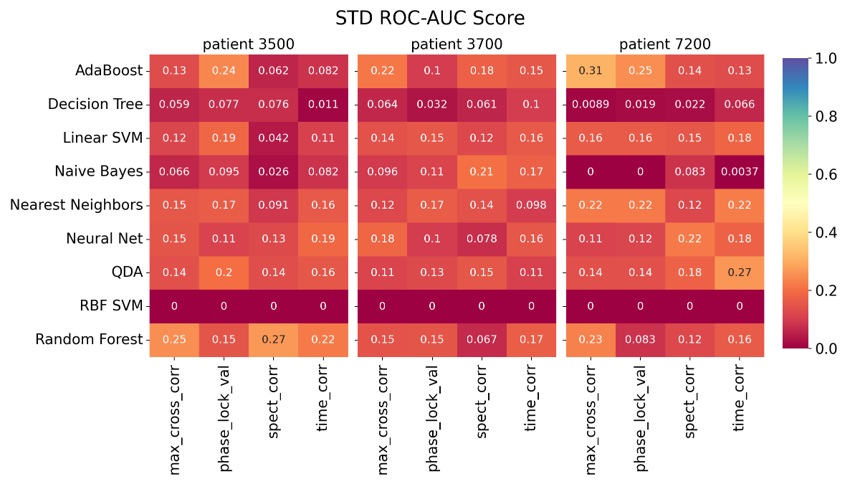
\includegraphics[width=\textwidth]{c2Deterministic/Figs/PSP/std_roc_auc_classifiers_and_features.png}
    \Caption{Standard deviation of AUC-ROC scores for 5-fold cross validation.}{}
    \label{fig:c2:std_roc_auc}
\end{figure}


\subsection{Training Efficiency}
Figure \ref{fig:c2:training_times} shows the mean time it took to fit each classifier to each feature-set, for each patient, over 5-fold CV. It is shown that the neural network, ensemble method (AdaBoost) and support-vector-machines consistently take longer than the decision tree, naive-Bayes, quadratic discriminant analysis, and random forest classifiers.

\begin{figure}[tb]
    \centering
    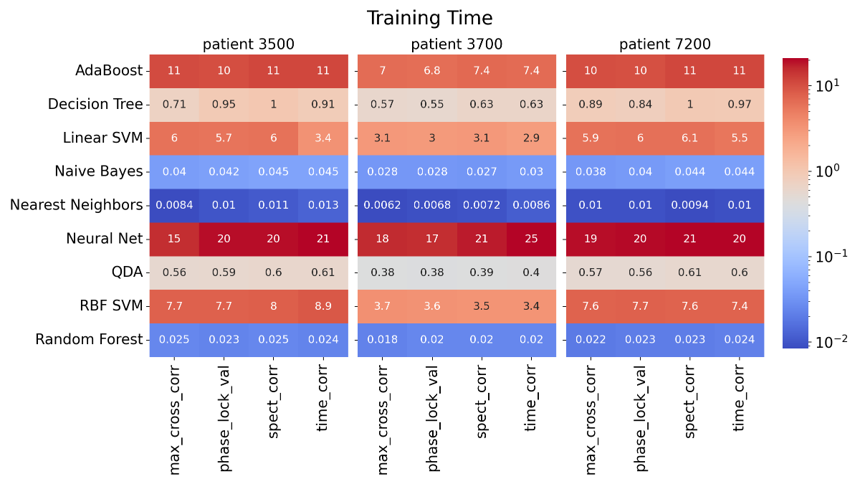
\includegraphics[width=\textwidth]{c2Deterministic/Figs/PSP/training_time_classifiers_and_features.png}
    \Caption{Mean training times (in seconds) for fitting the classifiers to the datasets.}{}
    \label{fig:c2:training_times}
\end{figure}

\subsection{Comparing Feature Sets}
The Linear SVM, which performed best in the previous experiments, is selected to compared the predictive performance of the different feature types. Notably, the classifier performed above chance in all feature sets, with the spectral correlation coefficients features slightly outperforming the others with respect to the ROC AUC score. See figures \cref{fig:c2det:350_svm,fig:c2det:370_svm,fig:c2det:720_svm}.

\begin{figure}[htp]
    \centering
    \subfloat[patient 3500]{%
      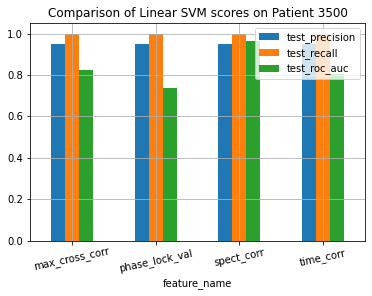
\includegraphics[clip,height=0.3\textheight]{c2Deterministic/Figs/PSP/pat_350_svm_features.png}
      \label{fig:c2det:350_svm}
    }

    \subfloat[patient 3700]{%
      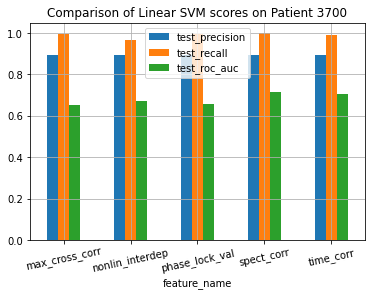
\includegraphics[clip,height=0.3\textheight]{c2Deterministic/Figs/PSP/pat_370_svm_features.png}
    \label{fig:c2det:370_svm}
    }

    \subfloat[patient 7200]{%
      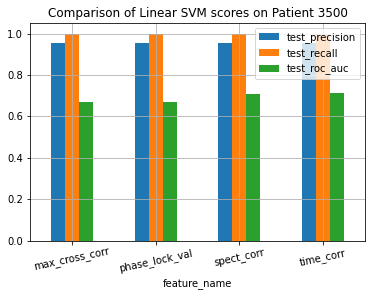
\includegraphics[clip,height=0.3\textheight]{c2Deterministic/Figs/PSP/pat_720_svm_features.png}
    \label{fig:c2det:720_svm}
    }

    \Caption{Results of Linear SVM on different feature datasets}{}

    % \begin{subfigure}[t]{}
    % \centering
    % 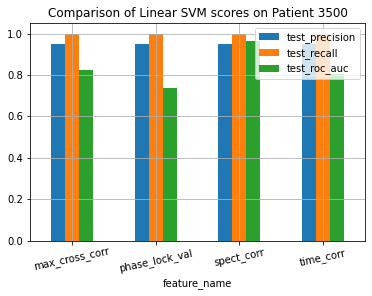
\includegraphics[height=0.3\textheight]{c2Deterministic/Figs/PSP/pat_350_svm_features.png}
    % \Caption{Comparison of predictive performance of Linear SVM for Patient 3500 on different feature datasets}{}
    % \label{fig:350_svm}
    % \end{subfigure}
    
    % \vfill
    % \begin{subfigure}[t]{}
    % 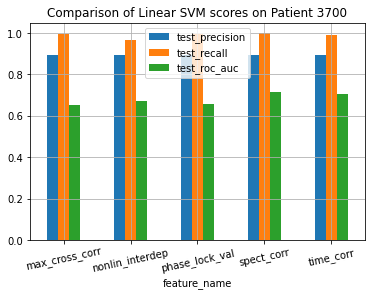
\includegraphics[height=0.3\textheight]{c2Deterministic/Figs/PSP/pat_370_svm_features.png}
    % \Caption{Comparison of predictive performance of Linear SVM for Patient 3700 on different feature datasets}{}
    % \label{fig:370_svm}

    % \end{subfigure}
    
    % \vfill
    
    % \begin{subfigure}[t]{}
    % 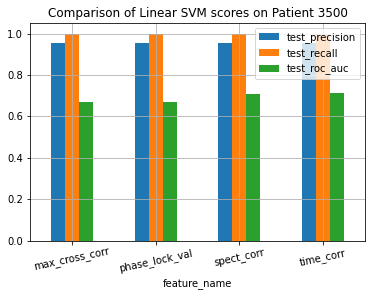
\includegraphics[height=0.3\textheight]{c2Deterministic/Figs/PSP/pat_720_svm_features.png}
    % \Caption{Comparison of predictive performance of Linear SVM for Patient 7200 on different feature datasets}{}
    % \label{fig:720_svm}
    % \end{subfigure}
    
\end{figure}


\section{Conclusion \& Discussion}

In this chapter, we explore the pattern recognition approach in a similar fashion to \citet{mirowski2009classification}, albeit on a newer dataset of noninvasive, 19 channel surface-EEG. We achieve comparable results across 3 subjects, with ROC-AUC scores commonly between 0.7-0.8 for a variety of bivariate feature sets related to inter-channel synchronicity with support vector machines.


\Citet{mirowski2009classification} evaluated their pipeline on 6-channel, intracranial data from 21 epilepsy patients. In this chapter, we use 19-channel data from surface EEG, from 3 patients. They reported 71\% sensitivity with 0 false alarms, on 15 out of the 21 patients they assessed. We trained 117 classifiers in different combinations of classifier-dataset. On the best classifier for each patient, only Patient 3700 achieves over 70\% sensitivity at the 0 false alarms threshold. For Patients 3500 and 7200, the sensitivities at 0 false alarms are 42\% and 40\%, respectively.

The main contribution of this chapter is to show that the classification of synchronicity-based features for seizure prediction is possible not just with intracranial data as in \cite{mirowski2009classification}, but also with surface-EEG from \citet{ihle2012epilepsiae}. Another difference between our data and the data analyzed in the previous work is the number of EEG-channels. Although the increase from 6 (15 pairs) to 19 (171 pairs) EEG channels gives us more sources of information, it also leads to a larger sample space such that probably much more data is needed.

This chapter showcases the predictive power of different classifiers and synchronicity-based features applied to noninvasive EEG data. We trained various classifiers. While some classifiers failed to generalize at all, most classifiers were successful in classifying better than chance, with AUC-ROCs in the range 0.67-0.81 commonly achieved. When comparing the synchronicity features, we did not find any of the feature sets to be remarkably better than the others in any of the 3 patients. 


% \begin{figure}[h]
%     \centering
%     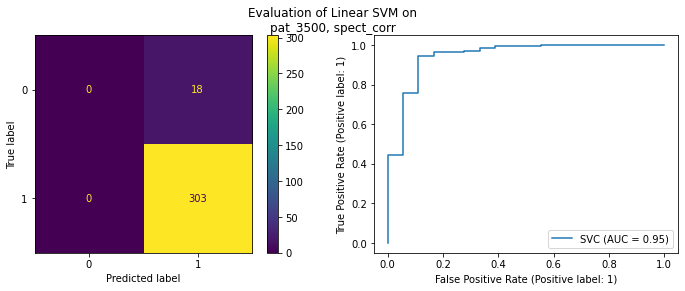
\includegraphics[width=\textwidth]{c2Deterministic/Figs/PSP/pat_350_best.png}
%     \caption{Plot of Confusion Matrix and ROC Curve for the highest scoring classifier for Patient 3500}
%     \label{fig:350_best}
% \end{figure}

% \begin{figure}[h]
%     \centering
%     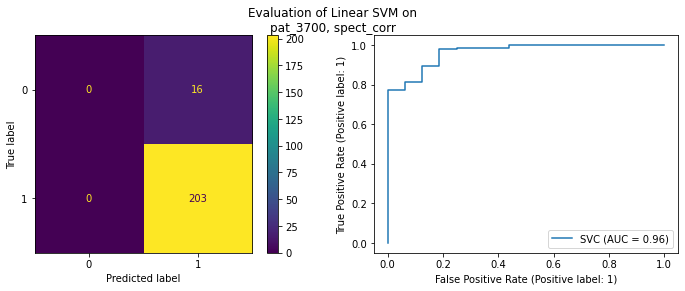
\includegraphics[width=\textwidth]{c2Deterministic/Figs/PSP/pat_370_best.png}
%     \caption{Plot of Confusion Matrix and ROC Curve for the highest scoring classifier for Patient 3700}
%     \label{fig:370_best}
% \end{figure}

% \begin{figure}[h]
%     \centering
%     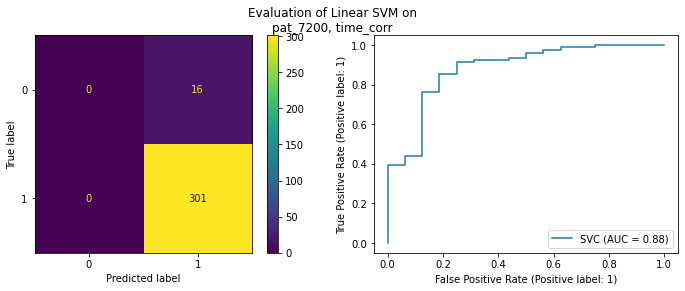
\includegraphics[width=\textwidth]{c2Deterministic/Figs/PSP/pat_720_best.png}
%     \caption{Plot of Confusion Matrix and ROC Curve for the highest scoring classifier for Patient 7200}
%     \label{fig:720_best}
% \end{figure}



% \newpage
